\chapter{Introducción}
En el presente capítulo se especifica la problemática que aborda la falta de disciplina y seguimiento en las actividades deportivas, enfocando el presente trabajo terminal en el arte marcial Karate Do. Así como la solución propuesta, el objetivo general y los objetivos específicos.
%------------------------------------------------------------------------------------
\section{Contexto}
Las actividades físicas y deportivas proveen salud física y mental, además de diferentes ventajas como la quema de calorías, la adopción de un estilo de vida saludable, la adquisición de una auto disciplina y de una mejor actitud, e incluso alcanzar cierta madurez mental \cite{Shotokan}. Muchos de los beneficios anteriores se obtienen principalmente en deportes como las artes marciales, ya que para estos se requieren largas horas de entrenamiento y práctica para alcanzar movimientos exactos y una perfecta coordinación; el Karate Do es una de las artes marciales más populares en el mundo.\\

Actualmente existen aplicaciones interactivas y de entretenimiento que fomentan las actividades físicas y deportivas, sin embargo como su meta es principalmente el entretenimiento, no toman en cuenta factores de salud del usuario y por tanto no se consideran un entrenamiento formal.\\

Para que el entrenamiento de Karate Do sea formal, se requiere de una educación reglamentada impartida por un responsable experto que pertenezca a una institución de manera oficial. Dicho responsable se encarga de enseñar, supervisar el desempeño del aprendiz, instruir aspectos como la disciplina e incluso  motivar; además de registrar los avances y realizar las observaciones pertinentes para corregir y mejorar el rendimiento del Practicante.\\

Gracias a las nuevas tecnologías de la información, la educación a distancia ofrece la posibilidad de estudiar y aprender sin necesidad de asistir presencialmente a un aula o a algún lugar definido. Teniendo como ventajas la atención personalizada, pues el instructor supervisa y corrige en la mayoría de los casos de manera individual; además de la flexibilidad de horarios, que facilita la administración del tiempo del aprendiz y el acceso al curso o servicio sin tener que recorrer grandes distancias, lo que supone un bajo costo.
%------------------------------------------------------------------------------------
\section{Problemática}
De acuerdo a un proceso de observación de las actividades de estudiantes, docentes y  al análisis documental realizado, hemos obtenido las siguientes problemáticas:

\begin{enumerate}
	\item Dificultades en el proceso enseñanza-aprendizaje. Para el entrenamiento de Karate Do, las personas necesitan tener iniciativa y constancia, sin embargo en estos días la gente tiende a reaccionar de forma apática cuando se les invita a entrenar o aprender, ya que asocian el entrenamiento o el aprendizaje con el aburrimiento,  actividades formales o incluso somnolientas \cite{Chye}.
	\item Falta de flexibilidad en horarios. Las personas tienen que trasladarse a un lugar determinado y ajustarse a un horario previamente programado.
	\item Falta de seguimiento de actividades por parte de entrenadores capacitados.
\end{enumerate}

Parte de los problemas previamente mencionados tienen relación o son comunes con la educación y aprendizaje en general, en los cuales la educación a distancia ha intervenido para solucionarlos.

%------------------------------------------------------------------------------------
\section{Solución propuesta}
La solución que se propone en el  presente trabajo terminal es desarrollar una herramienta de entrenamiento asíncrono a distancia que permita realizar un entrenamiento físico de Karate Do, tomando en cuenta ejercicios básicos de calentamiento aconsejados por la CONADE en sus programas de activación física, y técnica inicial de cinta blanca; permitiendo que el Practicante pueda realizar sus actividades en tiempo y forma en que le sea posible, y realizándose bajo la supervisión de un instructor experto. En el presente trabajo se tiene el apoyo y asesoría del experto Moisés Gachúz Mendoza cuyo grado es de Cinta Negra 5to Dan registrado en la Federación Mexicana de Karate Do desde el 2005.
Para el diseño de la solución propuesta se implementarán Interfaces Naturales de Usuario, debido a que los diferentes usuarios tienen concepciones distintas de la interacción con las computadoras, los cuales pueden ser diferentes en términos de cultura y cuyas preferencias cambian a través del tiempo \cite{Gomez}; utilizándolas para el manejo de la aplicación del Entrenador y Practicante durante la captura y validación de movimientos (ver sección \ref{sec:Alcance} \nameref{sec:Alcance}).\\

En la Figura \ref{fig:Bloques} \nameref{fig:Bloques} se presenta el diagrama a bloques de la herramienta propuesta.

\begin{figure}[H]%La h significa que la colocara cerca del texto
	\begin{center}
		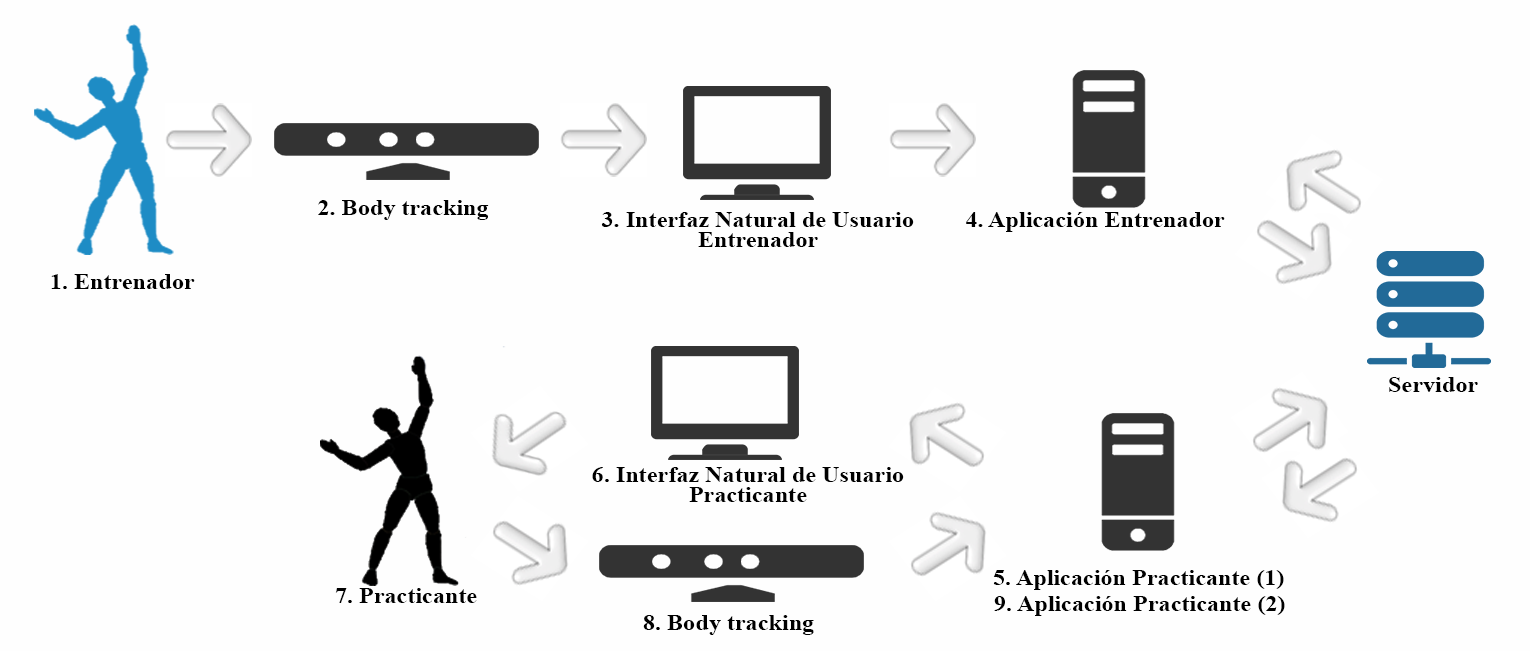
\includegraphics[scale=0.35]{./Figuras/DiagramaBloques}
	\end{center}
	\caption{Diagrama a bloques del diseño de la herramienta}
	\label{fig:Bloques}
\end{figure}

Proceso de la solución propuesta:

\begin{enumerate}
	\item \textbf{Entrenador.} Usuario especializado en Karate Do que registra los movimientos de la rutina de entrenamiento, además lleva un seguimiento del desempeño de los Practicantes. 
	\item \textbf{Body tracking.} El sensor Kinect realiza el seguimiento de los puntos del cuerpo del usuario los cuales son utilizados en la Interfaz Natural De Usuario Entrenador y en la Aplicación Entrenador. 
	\item \textbf{Interfaz Natural de Usuario Entrenador.} La interfaz con la que será mostrada y controlada la etapa de captura de movimientos de la interacción con los puntos obtenidos previamente por el sensor Kinect. 
	\item \textbf{Aplicación Entrenador.} 
	Con la información del body tracking obtenida por el sensor Kinect se realizará la captura de ejercicios y movimientos que el usuario Entrenador indique, teniendo en la aplicación un apartado con la gestión rutinas así como la gestión de los resultados de sus practicantes. 
	\item \textbf{Aplicación Practicante (1).} Recibe la información enviada por la aplicación Entrenador. 
	\item \textbf{Interfaz Natural de Usuario Practicante.} La interfaz con la que será mostrada y controlada la etapa de captura y validación de movimientos de interacción; además de mostrar los movimientos recibidos en la aplicación Entrenador. 
	\item \textbf{Practicante.} Usuario aprendiz en el entrenamiento del Karate Do quien recreará los movimientos de la rutina recibida del Entrenador. 
	\item \textbf{Body tracking.} El sensor Kinect realiza el seguimiento de los puntos del cuerpo del usuario los cuales son utilizados en la Aplicación Practicante. 
	\item \textbf{Aplicación Practicante (2).} Con la información del body tracking obtenida por el sensor Kinect se realiza la captura de ejercicios y movimientos del usuario Practicante, los cuales serán comparados con los movimientos recibidos realizados por el Entrenador, dando el resultado de su desempeño, mostrándolo en la Interfaz Natural de Usuario Practicante y enviándolo a través de internet a la aplicación Entrenador.
\end{enumerate}
%------------------------------------------------------------------------------------
\section{Objetivos}
\subsection{General}

Desarrollar una herramienta de software para el entrenamiento asíncrono a distancia (ver sección \ref{sec:elearning} \nameref{sec:elearning}) de la técnica inicial de cinta blanca de Karate Do (ver sección \ref{sec:Karate-Do} \nameref{sec:Karate-Do}), mediante el uso del sensor Kinect para el análisis de movimientos y para brindar apoyo en el seguimiento del desempeño del Practicante por parte del Entrenador.

\subsection{Específicos}
\begin{itemize}
	\item Delimitar los ejercicios de calentamiento de acuerdo a un organismo oficial.
	\item Delimitar los movimientos de la técnica inicial de cinta blanca de Karate Do.
	\item Definir los gestos y medios utilizados por el usuario para controlar la herramienta.
	\item Identificar y capturar  los movimientos del usuario.
	\item Implementar un mecanismo para la validación de movimientos.
	\item Implementar un medio de comunicación entre las aplicaciones de Entrenador y Practicante.
\end{itemize}
%------------------------------------------------------------------------------------
\section{Justificación}
Las estadísticas del INEGI reflejan el poco interés de los  mexicanos por realizar alguno de los que deportes que se ofertan, ya que de acuerdo a cifras recientes en ``deporte y ejercicio"  la tasa de participación en alguna actividad física-deportiva es de 43.8\%,  pero sólo el 30\% de la población lo práctica de manera regular o disciplinada, quienes en promedio invierten 3 horas 57 minutos a la semana \cite{INEGI}. Adicionalmente tomando como ejemplos las situaciones que se viven en otros países, como es el caso de España en el cual encuestas revelan que el principal resultado sobre la causa ó motivo por el cual las personas abandonaron algún deporte, fue el traslape de tiempos con sus actividades, sin embargo tenían en promedio 2-3 horas libres que les gustaría emplear practicando alguna actividad físico-deportiva. Los resultados también muestran que el aspecto que más influye o ayudaría para volver a practicar alguna actividad físico-deportiva es ``tener un monitor o Entrenador bien preparado" \cite{Efdeportes}.\\

Retomando la situación de nuestro país, con respecto a la elección del lugar donde se practica deporte, 49\% de los encuestados manifestaron que está relacionada sobre todo con la cercanía, un 17\% considera que lo ha elegido dado que cuenta con entrenadores confiables y un 14\% con el hecho de que se paga un precio accesible \cite{UVM}. Estos resultados muestran que se podría impulsar a las personas proporcionándoles los medios para que practiquen o continúen la actividad físico-deportiva de su agrado.\\

Existen aplicaciones comerciales que fomentan las actividades físico-deportivas, que permiten a los usuarios realizar una serie de rutinas programadas donde solamente se validan los movimientos de la rutina y se da un puntaje en base al desempeño, sin llegar a ser una disciplina formal, y en la mayoría de los casos no teniendo en cuenta la salud del usuario, al no realizar ejercicios previos de calentamiento.\\

En base a estas observaciones se ha determinado que a las personas les sería útil una aplicación donde un Entrenador dé indicaciones y pueda monitorear el desempeño del Practicante, pues el Entrenador es el experto que conoce los ejercicios que está enseñando. Una característica adicional de la aplicación que se plantea desarrollar es la retroalimentación profesor-alumno de los errores cometidos por el Practicante, dando instrucciones  de corrección y/o sugerencia.\\

Debido a que se hará la captura de movimientos de un Entrenador, y por medio de la interfaz natural de usuario, el estudiante replicará los movimientos; es posible que cualquier institución adopte este sistema, pero en el presente trabajo terminal se ha delimitado al entrenamiento de la técnica del Karate Do.